\documentclass[lang=cn,10pt,green]{elegantbook}
\usepackage{float}
\usepackage{subfigure}
\usepackage[normalem]{ulem} % \sout{想加删除线的中文}
\usepackage{wrapfig}
\usepackage{extarrows}
\newcommand{\incfig}[1]{%
\def\svgwidth{\columnwidth}
\import{./figures/}{#1.pdf_tex}
}



\renewcommand{\proofname}{\indent Pr}

\newcommand{\argmin}[1]{\underset{#1}{\arg \min}\ }
\newcommand{\ceil}[1]{\left\lceil #1 \right \rceil }
\newcommand{\norm}[1]{\left \Vert #1 \right \Vert}
\newcommand{\tform}[1]{\left \Vert #1 \right \Vert_2}
\newcommand{\tnorm}[1]{\left \Vert #1 \right \Vert_2}
\newcommand{\onorm}[1]{\left \Vert #1 \right \Vert_1}
\newcommand{\abs}[1]{\left|#1 \right|}
\newcommand{\var}[1]{\text{Var}\left[ #1\right]}
\newcommand{\xk}[1]{\left( #1\right)} 
\newcommand{\zk}[1]{\left[ #1\right]} 
\newcommand{\dk}[1]{\left\{ #1\right\}} 
\newcommand{\bd}[1]{\bold{#1}}

%量子力学符号------
\newcommand{\xde}{\text{Schrödinger}}
\newcommand{\avg}[1]{\left \langle #1 \right \rangle}
\newcommand{\lvec}[1]{\left \langle #1 \right |}
\newcommand{\rvec}[1]{\left | #1 \right \rangle}


\newtheorem{lproof}{证明}[section]
\newtheorem{tuilun}{推论}
\newtheorem{eg}{例}[section]
\newtheorem{solve}{解}[section]
\newcommand\ii{\textup{i}}
\newcommand\dd{\mathrm{d}}


%自定义数学符号
\newcommand{\diag}{\textup{diag}}
\newcommand{\Frobenius}[1]{\left\Vert #1 \right\Vert}
\newcommand{\fform}[1]{\left\Vert #1 \right\Vert_F}
\newcommand{\parr}[2]{\frac{\partial #1}{\partial #2}}%一阶偏微分
\newcommand{\parrr}[2]{\frac{\partial^2 #1}{\partial #2^2}}%二阶偏微分
\newcommand{\lap}[1]{\parrr{#1}{x} + \parrr{#1}{y} = 0}%二元拉普拉斯方程
\newcommand{\ddd}[2]{\frac{\textup{d} #1}{\textup{d} #2}}%微商
\newcommand{\dddd}[2]{\frac{\textup{d}^2 #1}{\textup{d} #2^2}}%微商

%二重以上环路积分,强迫症了属于是
\def\ooint{{\bigcirc}\kern-11.5pt{\int}\kern-6.5pt{\int}}
\def\oooint{{\bigcirc}\kern-12.3pt{\int}\kern-7pt{\int}\kern-7pt{\int}}


\newcommand{\tu}{\textup}
\newcommand{\ol}[1]{$\overline{#1}$}
\newcommand{\re}[1]{\textup{Re}(#1)}
\newcommand{\im}[1]{\textup{Im}(#1)}
\newcommand{\fa}{\forall}
\newcommand{\ex}{\exists}
\newcommand{\st}{\textup{  s.t. }}
\newcommand{\ve}{\varepsilon}
\newcommand{\disp}{\displaystyle}
\newcommand{\chj}{\textup{Cauchy}积分公式}
\newcommand{\res}[1]{\textup{Res}\left(#1\right)}
\newcommand{\mysum}[1][n]{\sum_{i = 1}^{#1}}%求和
\newcommand{\series}[1]{\sum_{n = 0}^{\infty} #1_{n}}%级数
\newcommand{\seriesa}[1]{\sum_{n = 0}^{\infty} \left| #1_{n}\right|}%绝对级数
\newcommand{\fseries}[1]{\sum_{k = 1}^{\infty} #1_k (z)}

\newcommand*{\num}{pi}

%书写横线
\newcommand{\horrule}[1]{\rule[0.5ex]{\linewidth}{#1}} 	% Horizontal rule

\title{Introduction to Computer Vision Notes}
\subtitle{授课教师:\href{https://hughw19.github.io}{王鹤}}
\author{林晓疏, \href{https://lyt0112.com/}{梁宇桐}, \href{https://iculizhi.github.io/}{徐靖}}
\institute{PKU EECS}
\version{2025 Spring}
\bioinfo{声明}{\textcolor{red}{请勿用于个人学习外其他用途!}}
\extrainfo{个人笔记,如有谬误,欢迎指正!\\ 联系方式:2200012917@stu.pku.edu.cn}

\setcounter{tocdepth}{3}

% 自定义封面元素
\cover{cover.jpg}
\logo{logo-blue.png}

% 本文档命令
\usepackage{array}
\newcommand{\ccr}[1]{\makecell{{\color{#1}\rule{1cm}{1cm}}}}

% 修改标题页的橙色带
% \definecolor{customcolor}{RGB}{32,178,170}
% \colorlet{coverlinecolor}{customcolor}
\setcounter{tocdepth}{3} % 设置目录深度
\begin{document}

\maketitle
\frontmatter

\tableofcontents

\mainmatter

\chapter{Line Fitting}

\section{Least Square Method}

\begin{figure}[htbp]
    \centering
    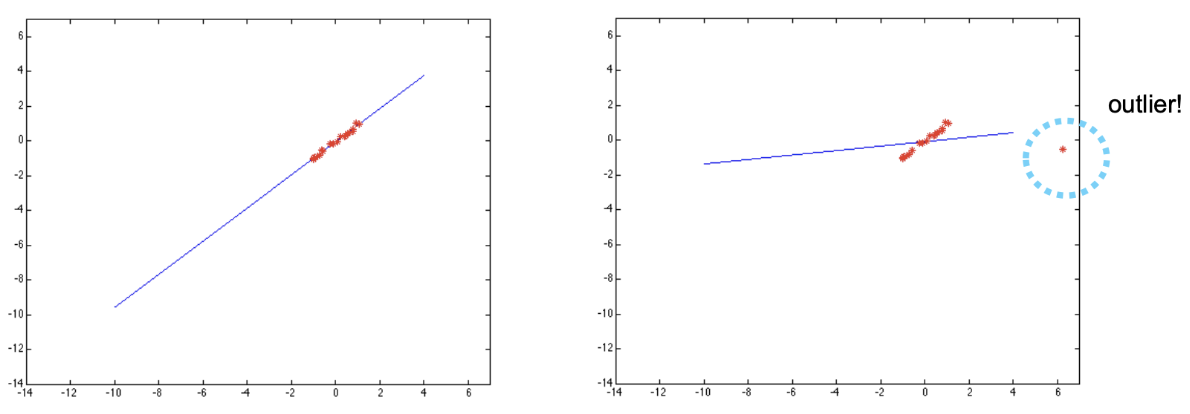
\includegraphics[width=0.8\textwidth]{figures/not_roboust_outliner.png}
    \caption{Least Square Method is not robust to outliers}
\end{figure}

对细微噪声鲁棒(robust), 但是对于离群点(Ouliers)敏感.

\section{RANSAC}

RANSAC:RANdom SAmple Consensus

Idea: we need to find a line that has the largest supporters (or inliers)

RANSAC loop:

假设这个直线 (平面) 需要两个 (n个) 点来确定.

\begin{enumerate}
    \item 随机选择 k 组能确定这个直线的点,也就是在所有点里面选出一个 $k\times 2$ 的矩阵
    \item 对每一组点计算出一条直线
    \item 对每一组点的直线计算出所有点到这条直线的距离,如果小于阈值,则认为这个点是这条直线的 inlier
    \item 找到最大的 inlier 数量的直线,如果大于阈值,则认为这条直线是最优的
    \item 对这个最优的直线,用这个直线所有的 inlier 重新计算一次直线
\end{enumerate}

\section{RANSAC calculation}

假设我们有所有 inliner 占比为 $w$ 的先验知识,同时希望有不低于 $p$ 的概率能够找到一个最优的直线,那么我们需要多少次迭代呢?

\begin{equation}
\mathbf{\Pr}\text{[一组点全部是inliner]} = w^n
\end{equation}

如果一组点中有一个点是 outliner,那么我们称这组点 fail.

\begin{equation}
\mathbf{\Pr}\text{[k组点全部fail]} = {(1-w^n)}^k
\end{equation}

我们希望 k 组点全部 fail 的概率小于 $1-p$.

\begin{equation}
{(1-w^{n})}^k < 1-p
\Rightarrow
k > \frac{\log(1-p)}{\log(1-w^n)}
\end{equation}

\section{Hough Transform}

其实就是把一条直线从实际空间的表示转换到参数空间的表示.但是如果存在垂直的直线,可能需要考虑使用极坐标来作为参数空间.

\begin{figure}[htbp]
    \centering
    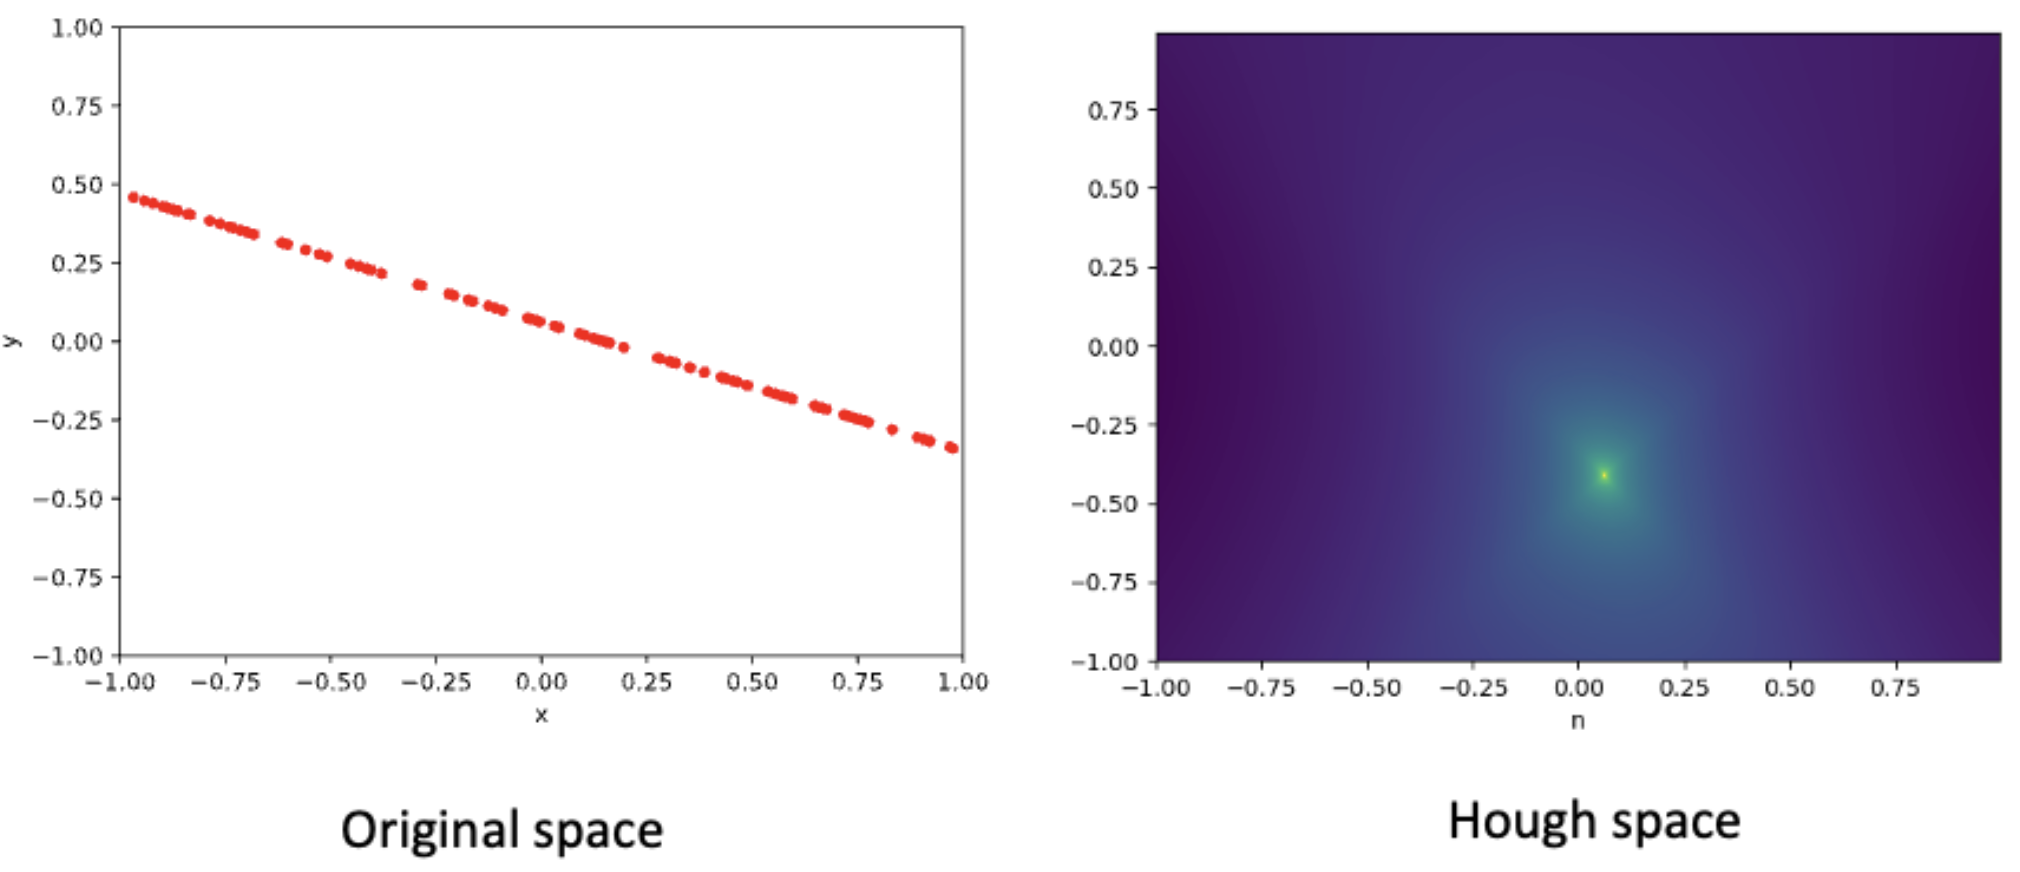
\includegraphics[width=0.8\textwidth]{figures/hough1.png}
    \caption{Hough Transform w/o Noise}
\end{figure}

\begin{figure}[htbp]
    \centering
    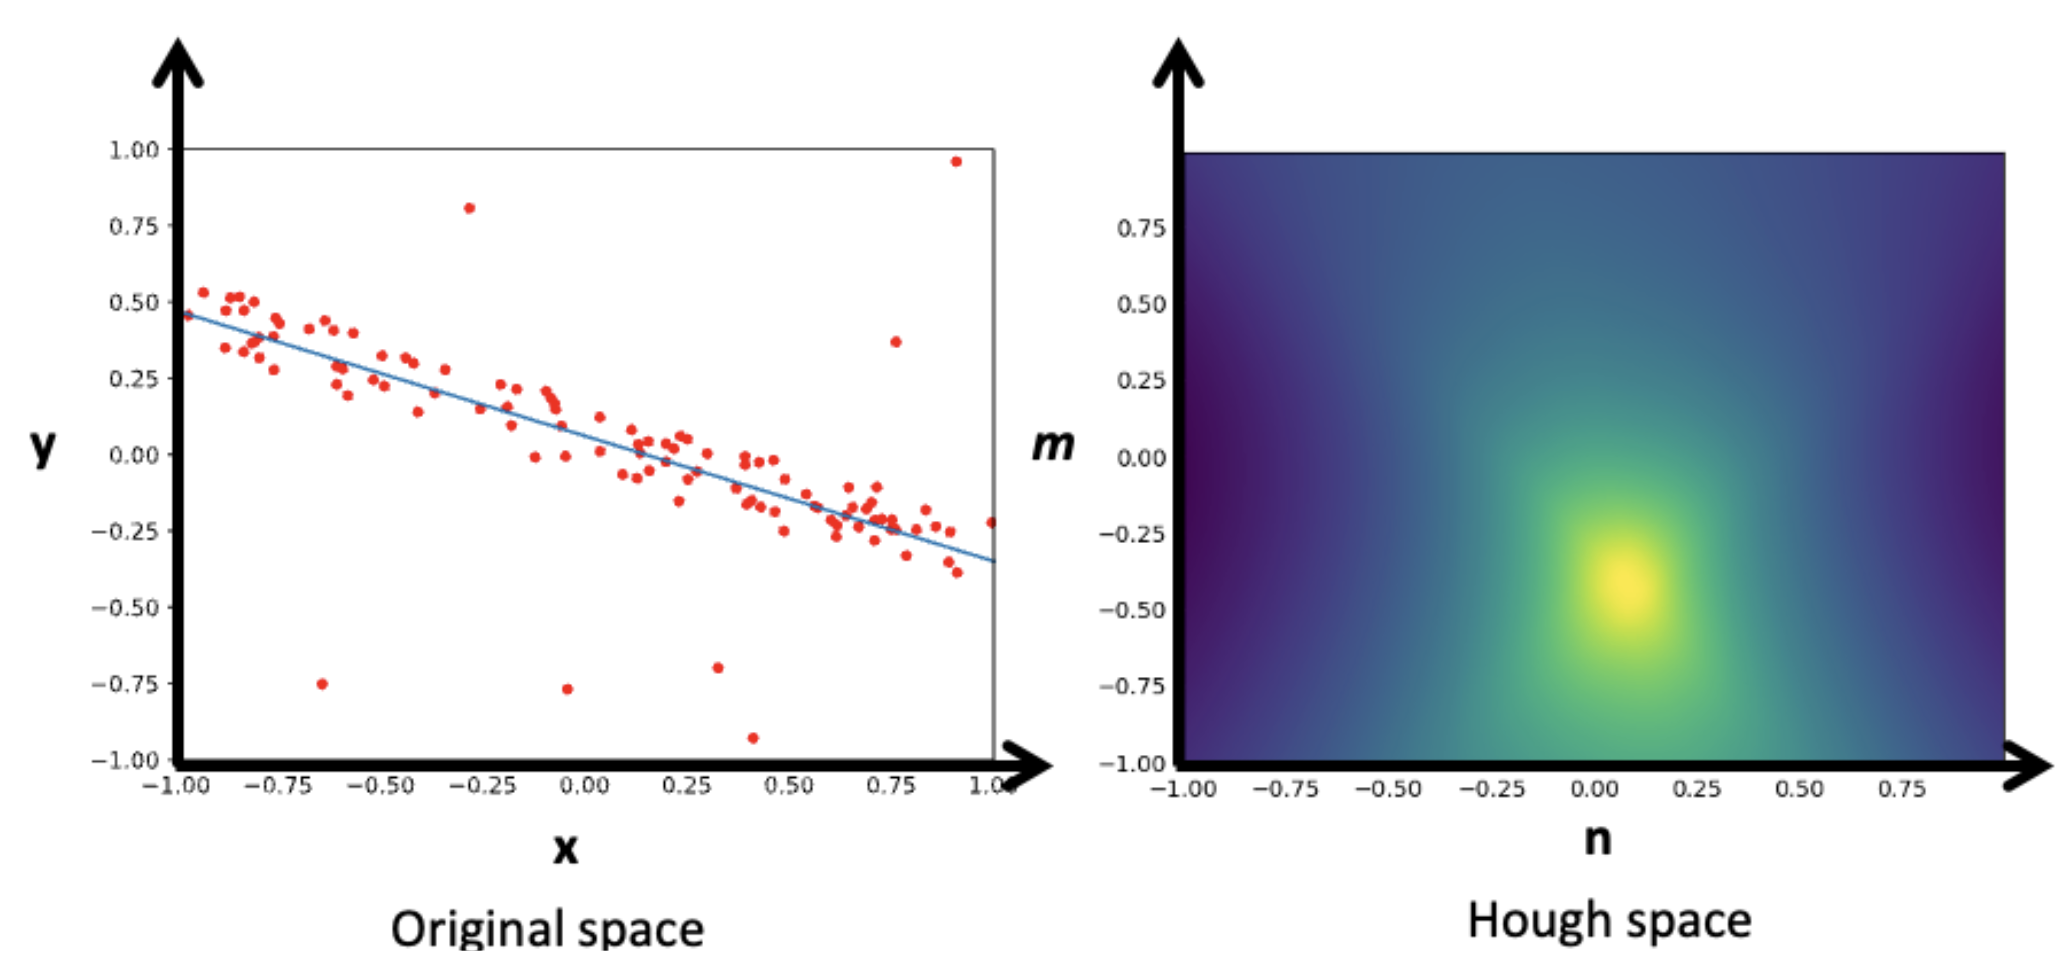
\includegraphics[width=0.8\textwidth]{figures/hough2.png}
    \caption{Hough Transform w/ Noise and Outliers}
\end{figure}


\printbibliography[heading=bibintoc, title=\ebibname]
\end{document}
